\chapter{Correlation Analysis}
\label{chpr:corr_analysis}
In order to get an initial insight on how Bitcoin is correlated with other assets, we will perform a correlation analysis based on the empirical time series of our data. We will focus our attention on the logarithmic returns it is the standard practice. We will often refer to logarithmic returns simply as returns, only specifying their nature when it is necessary to avoid confusion.


\bigskip

\section{Empirical Correlation of Returns}
\label{emp_corr}

We first start by performing some statistical analysis on the data in order to estimate the distribution from which they are sampled.
For this part, we will consider our data as successive samples of a $N$-dimensional vector in $\mathbb{R}^{N}$, where $N$ is the number of assets:
\begin{equation*}
	\mathbf{x}_{j}\\
	 = \begin{pmatrix}
	x_{1,j} \\
	x_{2,j}	\\
	\vdots\\
	x_{N,j}
	\end{pmatrix} , j = 1 \dots N_{sample}
\end{equation*}
Each element $i$ of the vector $\mathbf{x}_j$ represents the $j^{th}$ realization of the returns for asset $i$.

Following basic statistics, we can now compute the \textit{sample mean} of our vectors of returns as:
\begin{equation*}
	\mathbf{\bar{x}} = \frac{1}{N_{sample}} \sum_{j=1}^{N_{sample}} \mathbf{x}_j =
	\begin{pmatrix}
	\bar{x}_{1} \\
	\bar{x}_{2}	\\
	\vdots\\
	\bar{x}_{N}
	\end{pmatrix}
\end{equation*}
where $\bar{x}_{i} = \frac{1}{N_{sample}} \sum_{j=1}^{N_{sample}} x_{i,j}$ is the sample mean of component $i$.

Now we compute the \textit{sample covariance matrix} through the following formula:
\begin{equation*}
\bar{\Sigma}  = \frac{1}{N_{sample}-1} \sum_{j=1}^{N_{sample}} (\mathbf{x}_j - \mathbf{\bar{x}}) (\mathbf{x}_j - \mathbf{\bar{x}})^T
\end{equation*}
where $\mathbf{\bar{x}}$ represent the sample mean of the returns just introduced.
	
All the information needed to obtain the \textit{correlation matrix} $C$ are already included in $\bar{\Sigma}$, we only need to perform some further calculations:
\begin{equation}
\label{corr_eq}
	C_{i,j} = \frac{\bar{\Sigma}_{i,j}}{\sqrt{\bar{\Sigma}_{i,i} \bar{\Sigma}_{j,j}}}
\end{equation}

We have thus obtained an empirical estimate of the correlation between our assets returns. The formula in (\ref{corr_eq}) is often referred to as \textit{Pearson correlation coefficient}, from the name of the English mathematician Karl Pearson who first formulated it.

Results are reported in the following tables.

\begin{center}
	\textbf{****** ADD RESULT TABLES ******}
\end{center}

We are mainly interested in the correlation between Bitcoin and other assets returns, so we will now focus on the first row (or equivalently column, by symmetry) of the correlation matrix.

All values are fairly close to zero, never exceeding $10\%$ towards the positive or the negative side. 
One may thus wonder whether these correlations are \textit{statistically significantly} different from zero.
To answer this question, we will introduce two statistical tests to check the correlation significance.


\bigskip
\section{Correlation Significance}
The very core of Inferential Statistics, the branch of statistics that allows to draw conclusions from the information contained in a set of data, is hypothesis testing. 

In our case, we are specifically interested in testing if the sample correlation coefficients are significantly different from zero or not.
Both of the following tests are presented in the most general form for a sample of two variables, their distribution correlation $\rho$ and their sample correlation $\hat{\rho}$. 

Following standard testing procedure, we specify the \textit{null hypothesis} and the \textit{alternative hypothesis}:
\begin{equation*}
	\mathbf{H_{0}}: \quad \rho = 0 \quad vs. \quad	\mathbf{H_{1}}: \quad \rho \neq 0
\end{equation*}
These will be common to both presented tests.

\subsection{\textit{t}-test}
Our first test is based on Student's t-distribution and the following t-statistic:
\begin{equation}
	t = \hat{\rho} \sqrt{\frac{n - 2}{1 - \hat{\rho}^2}}
\end{equation} 

which under the null hypothesis is distributed as a Student's $t$ with $n-2$ degrees of freedom, where $n$ stands for the cardinality of the sample.
We can thus proceed by computing the relative p-value and compare it to a given level of confidence $\alpha$ (usually $\alpha = 95\%$). 
The result of the test will be deduced as follows:
\begin{itemize}
	\item $p-value < 1 - \alpha$ : we have statistical evidence to state that the correlation is \textit{significantly} different from zero;
	\item $p-value \geq 1 - \alpha$ : there is \textit{no statistical evidence} to state that the correlation is different from zero.
\end{itemize}


\subsection{Permutation test}
 The permutation test is based on building an empirical distribution of values for the correlation by sampling different pairs of $X$ and $Y$ variable and then computing Pearson's correlation. If this is done a large enough number of times, we obtain an empirical distribution of possible values. 
 From this distribution we can then obtain the p-value of the test and thus the final result in the same way as in the previous case.
 

\subsection{Significance results}
 
 ********Comments and numerical results***************
 
 \bigskip
\section{Rolling Correlation}
Our study so far has focused on the analysis of the dataset as a whole, with values spanning from 2010 to 2018. This is clearly  important if we want to obtain a general overview of the period, but it is also interesting to see how the correlation between the  assets has evolved through. 
Therefore, we present in Figure \ref{roll_corr} the results obtained from calculating the correlation between Bitcoin and the other assets using  rolling windows of 36 and 18 months, updated monthly.


\begin{figure}
	\centering
	\begin{subfigure}{\textwidth}
		\centering
		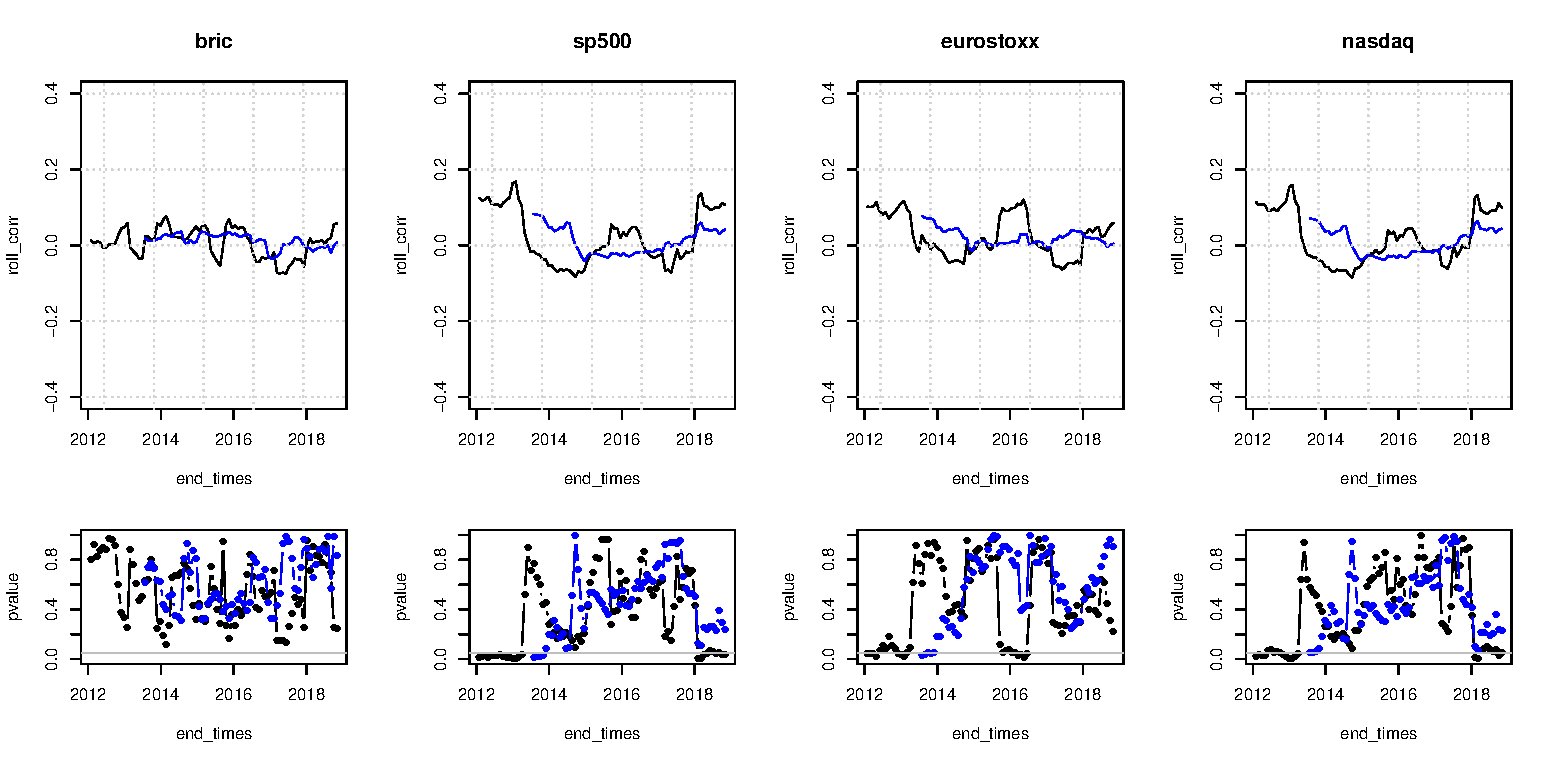
\includegraphics[width=0.8\linewidth]{Images/rolling_stocks}
		\label{roll_stocks}
		\caption{Stocks}
	\end{subfigure}\\

	\begin{subfigure}{0.66\textwidth}
		\centering
		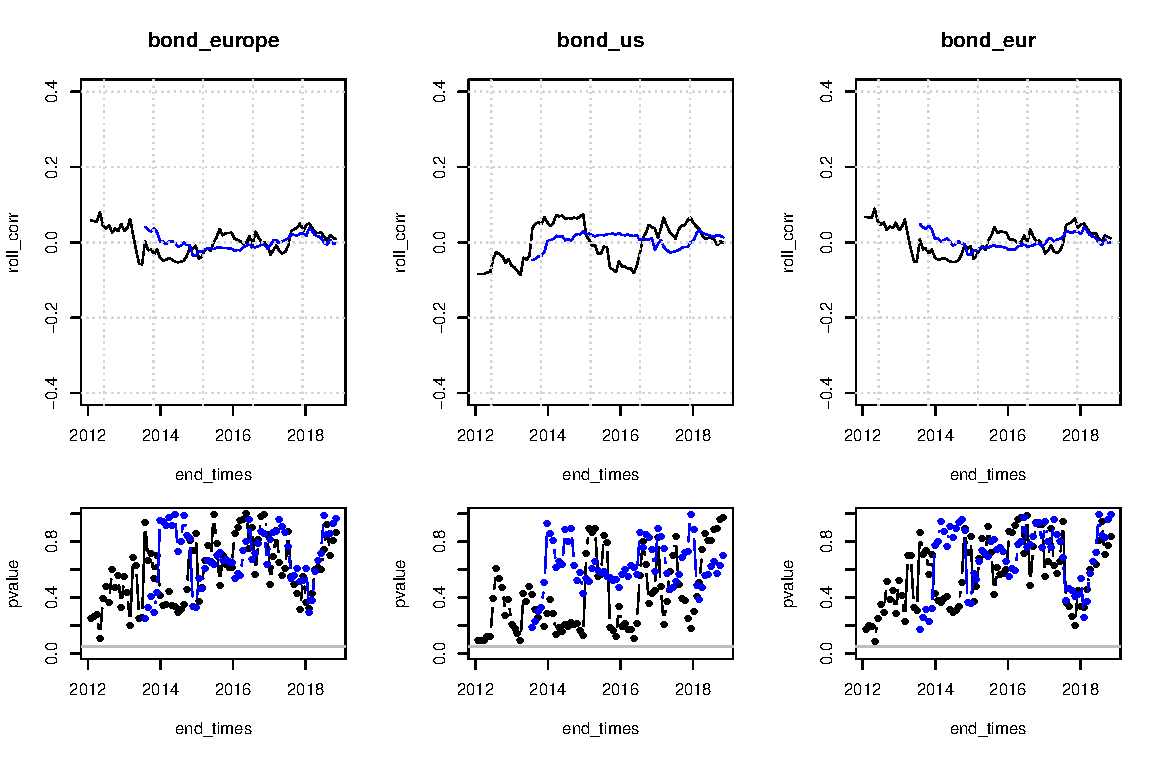
\includegraphics[width=0.8\linewidth]{Images/rolling_bonds}
		\caption{Bonds}
		\label{roll_bonds}
	\end{subfigure}\\
	\begin{subfigure}{\textwidth}
		\centering
		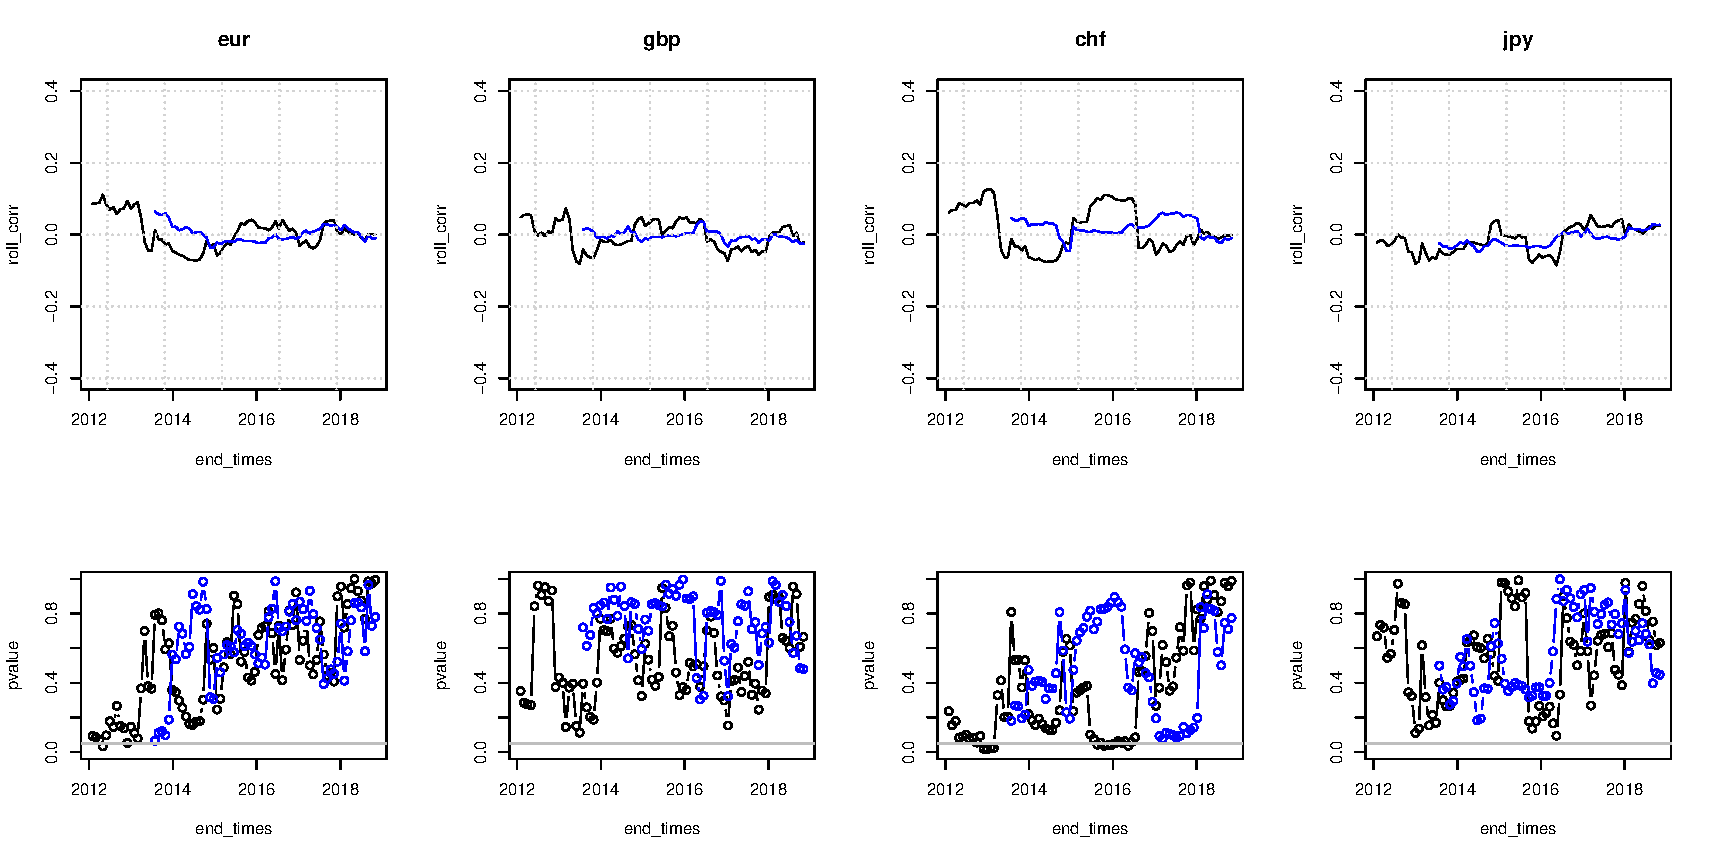
\includegraphics[width=0.8\linewidth]{Images/rolling_fx}
		\caption{Currency exchange}
		\label{roll_currencies}
	\end{subfigure}
	\begin{subfigure}{\textwidth}
		\centering
		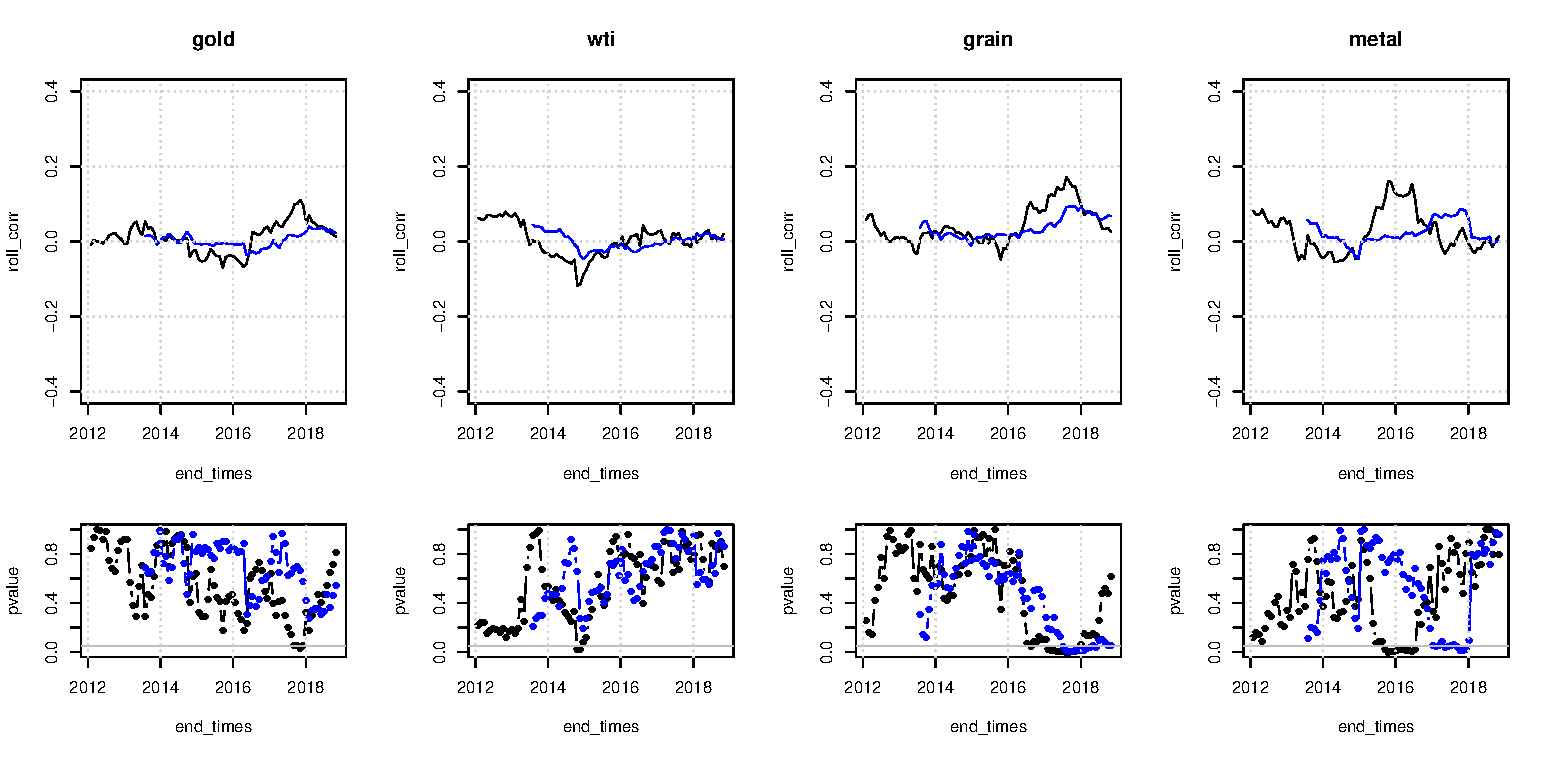
\includegraphics[width=0.8\linewidth]{Images/rolling_commodities}
		\caption{Commodities}
		\label{roll_commodities}
	\end{subfigure}
	\caption{Plots of rolling correlation for the different asset classes (on top) and significance for each value (on bottom). Blue lines are the 3-year rolling correlations, while the black ones have a window of 18 months. Both computations are updated monthly.}
	\label{roll_corr}
\end{figure}


There are two graphs for each asset: in the top plots levels of the rolling correlations are represented using two different colours, blue for the 3-year and black for the 18-month windows; in the bottom plots we included the significance of each rolling correlation through its p-value. The grey horizontal line represents the 5\% level of significance\footnote{As we explained in the previous section, to check that a sample correlation is \textit{significantly} non zero, we compare the p-value of the test to a given level, here $1- \alpha$ = 5\%. Graphically, whenever the dots are above the grey line in Figure \ref{roll_corr}, the corresponding correlation is \textit{not} significantly different from zero.}. 

The main conclusion we can draw from these images is that the correlation of any asset with Bitcoin is hardly ever significantly different from zero, and when it is, its absolute level is never more than greater than 20\% for a small period of time.

To confirm the fact that Bitcoin is not correlated with any asset, we can also take a look at the path of the rolling correlations: there is no line that is always above zero, nor below. This indicates that there is no underlying trend, whether positive or negative, and the correlation one might find is only temporary.

**** maybe add more comments on the results ****



